\section{Office building load profile}

For nearly energy-neutral buildings (bijna energieneutrale kantoorgebouwen 'BENG') specific requirements for energy consumption will apply from 2021.The maximum energy requirement for heating, cooling and lighting for utility buildings, is 50 kWh/$m^2$ per year. The number is increased to 65 kWh/$m^2$ per year for healthcare buildings.This excludes the energy consumption for office equipment \cite{Benchmark1}.\\
The average gas consumption for office building is around 17 $m^3$/$m^2$ (figure 1) for the building with the construction year between 1977 and 1989.The report from ECN has calculated the buildings with an office function cover a total of 87 million m2. This concerns 68,000 buildings in the Netherlands. Gas consumption amounts to 955 million m3 (30 PJ) and electricity to 7800 million kWh (28 PJ). These values are the most accurate available at the moment \cite{Benchmark2, ECN}.

\begin{figure}[ht]
\centering
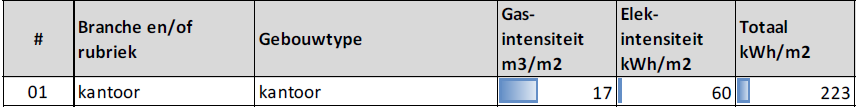
\includegraphics[width=1\columnwidth]{pictures/ECN.png}
\caption[Short title]{Energy Consumption}
\label{fig:consumption}
\end{figure}

% \begin{figure}[ht]
% \centering
% 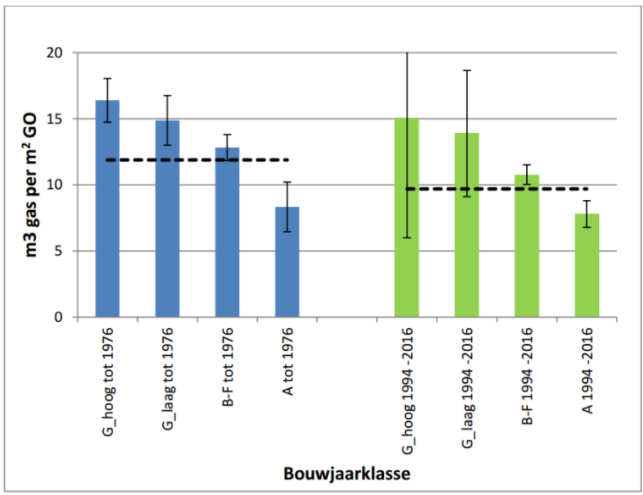
\includegraphics[width=1\columnwidth]{pictures/gas use.png}
% \caption[Short title]{Office building gas consumption per m2 }
% \label{fig:ff1}\end{figure}

The reference building has been selected:

\begin{itemize}
  \item Construction year: 1977-1989.
  \item Surface $m^2$: 500
  \item Gas consumption: 17 $m^3$/$m^2$
  \item T{\_outside} : out door temperature from NEN5060\texttt{\_}2018 with 1 hour sampling rate for 1 year long.
\end{itemize}
    
Add plot of load profile .... and validate



% Assume that there is no heating needed, when out side temperature is 15 degree. The heating line is set on 14 $^o$C.
% The office is 500 $m^2$ the gas consumption is around 8500  $m^3$ gas or 82450 kwh (1 $m^3$ equals approximately 9.7 kWh).\\
% The (“graaduren”) $^o$C per hour necessary to achieve the right inside temperature.


% %\[Q_{per{\_}degree} = \frac{97000}{\sum{(14 - T_{outside})}}\] 

% \begin{equation}
% Q_{per{\_}degree}=\frac{97000}{\sum(14 - T_{outside})}
% \end{equation}

% Energy demand profile is calculated with period of 1 hour for the whole year.

% \begin{equation}
% Q_{profile}=Q_{per{\_}degree}*{(14 - T_{outside})}
% \end{equation}

% The energy demand profile is showed in figure 1.

% \begin{figure}[H]
% \centering
% 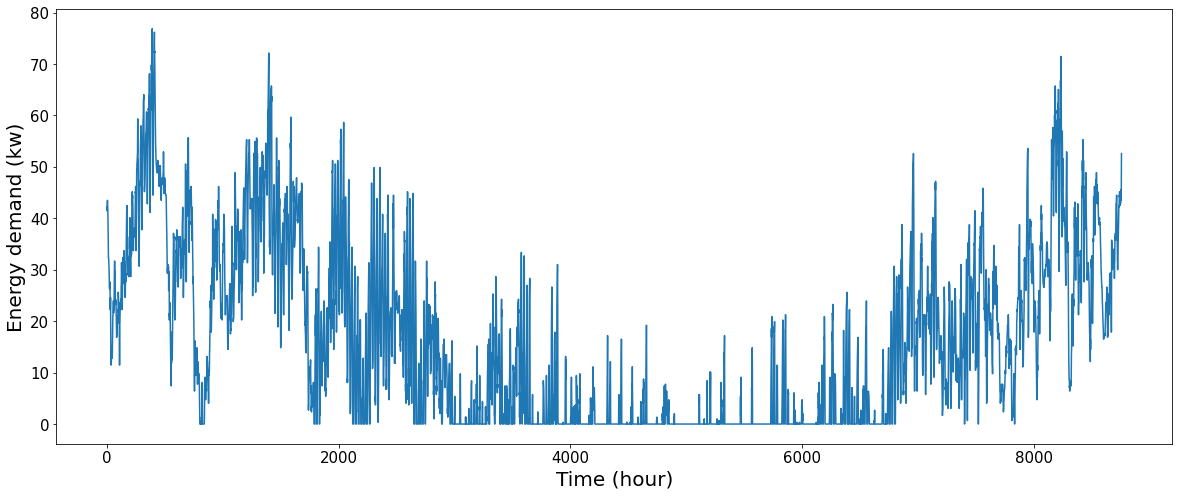
\includegraphics[width=1\columnwidth]{pictures/Q_profile.png}
% \caption[Short title]{Energy Consumption of office building.}
% \label{fig:ff2}\end{figure}

